% !Mode:: "TeX:UTF-8"
%% 请使用 XeLaTeX 编译本文.
\documentclass{WHUResearch}  % 选项 forprint: 交付打印时, 建议加上此选项, 以消除彩色链接文字, 避免彩色字迹打印偏淡.
                             % 选项 forlib: 提交给图书馆的电子版, 需要加上选项 forlib, 以消除空白页和彩色链接.
                             % 选项 smd: Specialist Master's Degree, 产生专业硕士学位论文封面、页眉.                                                                                                   
%%%=== 参考文献=== %%%
\bibliographystyle{abbrv}    % 参考文献样式,  plain,unsrt,alpha,abbrv 等等
%%%%%%%%%%%%%%%%%%%%%%%%%%%%%%%%%%%%%%%%%%%%%%%%%%%%
\begin{document}
%%%%%%%-------------------------------------------------

\title{Nordic nRF5 开发文档}
\author{钱隆}
\StudentNumber{2019106190015}   % 学号

%-----------------------------------------------------------------------------
\pdfbookmark[0]{封面}{title}         % 封面页加到 pdf 书签
\maketitle
%-----------------------------------------------------------------------------
\pagenumbering{Roman}               % 正文之前的页码用大写罗马字母编号.

\cleardoublepage
\newpage  \pagestyle{fancy} \fancyfancy
%------------------------------------------------------------------------------
%---把目录加入到书签---%%%%%%%%%%%%%%
\pdfbookmark[0]{目录}{toc}%%%%%%%%%%%%

\tableofcontents

%------------------------------------------------------------------------------
\mainmatter %% 以下是正文
\baselineskip=20pt  % 正文行距为 20 磅
\zihao{-4}
%%%%%%%%%%%%%%%%%%%%%%%%%%%%%%%%%%%%
\chapter{Nordic nRF5系列产品开发流程}

These sections will guide you through choosing the right protocols to production programming and testing your product design.

\section{Available protocols}




\chapter{Nordic nRF5系列软件开发环境搭建}

\section{Windows平台基于ARM Keil MDK开发环境搭建}

本节参考\href{https://www.cnblogs.com/iini/p/9043565.html}{iini的博客} \upcite{BKY_iini} 以及 Nordic 的官方入门教程 \href{https://infocenter.nordicsemi.com/index.jsp?topic=\%2Fug_gsg_keil\%2FUG\%2Fgsg\%2Fintro.html&cp=1_1_1}{nRF5 Series: Developing on Windows with ARM Keil MDK},记录在 Windows 平台上基于 ARM Keil MDK 进行 nRF5 系列开发软件环境的准备工作,为今后基于该芯片的开发提供指导。

首先简要介绍一下软件开发环境的依赖项包括:ARM C/C++ 编译器(Compiler),µVision 集成开发环境(Integrated Development Environment)以及 Nordic 官方提供的 nRF5 软件开发工具包(Software Development Kit)。本节所记录的开发环境配置基于 nRF52811 。

\subsection{基础环境配置要求(Minimum Requirements)}

$\bigstar$ 硬件要求

nRF5 系列开发平台(Development Kit, DK)包括一块与之相对应的开发板以及开发板上的芯片。因为Nordic Semiconductor的一些软件开发工具会针对特定的开发板或芯片,所以在进行基于自定义开发板的软件开发之前,需要明确自定义开发板、芯片、SDK等组件的兼容性关系,以确保开发程序正确烧制到自定义开发板上。在相应芯片的说明文档中可以找到对应的兼容矩阵说明。

\href{https://infocenter.nordicsemi.com/index.jsp?topic=\%2Fcomp_matrix_nrf52811\%2FCOMP\%2Fnrf52811\%2Fnrf52811_comp_matrix.html&cp=3_2_2}{nRF52811 平台的兼容性矩阵}(Compatibility Matrix)信息如下:

$\star$ \href{https://infocenter.nordicsemi.com/index.jsp?topic=\%2Fcomp_matrix_nrf52811\%2FCOMP\%2Fnrf52811\%2Fnrf52811_ble_qdid_qual_matrix.html&cp=3_2_2_4}{集成电路修订和变量(IC revisions and variants)}
\begin{table}[htbp]
  \centering
  \caption{nRF52811 IC revisions and variants}
  \begin{threeparttable}
	\begin{tabular}{|c|c|c|c|c|c|}
	\hline
   \textbf{nRF52811 IC revision}  & \textbf{Packet variant}\tnote{1} & \textbf{Build code}\tnote{1} & \textbf{Package} & \textbf{Flash} & \textbf{RAM} \\ \hline
	\multirow{3}{*}{Engineering A} & QFAA 						   & \multirow{3}{*}{AA0} & QFN48 & \multirow{6}{*}{192kB} & \multirow{6}{*}{24kB} \\ \cline{2-2} \cline{4-4}
                  					  & QCAA                     &                   	& QFN32 &                   &                   \\ \cline{2-2} \cline{4-4}
                  					  & CAAA							&                   	& WLCSP &                   &                   \\ \cline{1-4}
	\multirow{3}{*}{\underline{1}} & QFAA							& \multirow{3}{*}{AX0} & QFN48 &                   &                   \\ \cline{2-2} \cline{4-4}
                  					  & \underline{QCAA	}			&                   	& \underline{QFN32} &                   &                   \\ \cline{2-2} \cline{4-4}
                 					  & CAAA							&                   	& WLCSP &                   &                   \\ \hline
	\end{tabular}
	\begin{tablenotes}
	  \footnotesize
        \item[1] Packet variant 和 Build code 可以通过 nRF52 芯片上的印刷标志(N52811 QCAAAA 1836AA)获得。
	\end{tablenotes}
  \end{threeparttable}
\end{table}

$\star$ \href{https://infocenter.nordicsemi.com/index.jsp?topic=\%2Fcomp_matrix_nrf52811\%2FCOMP\%2Fnrf52811\%2Fnrf52811_ble_qdid_qual_matrix.html&cp=3_2_2_4}{软件开发工具包和无线协议栈(SDKs and SoftDevices)}
\begin{table}[htbp]
  \centering
  \caption{nRF52811 IC revisions, nRF5 SDKs, and SoftDevices}
	\begin{tabular}{|c|c|c|c|}
	\hline
 	\multirow{2}{*}{\textbf{nRF52811 IC revision}} & \multirow{2}{*}{\textbf{nRF5 SDK}} &  \multicolumn{2}{c|}{\textbf{BLE}} \\ \cline{3-4}
 															  &  											 & \textbf{S112 SD} & \textbf{S112 SDS} \\ \hline
 	Engineering A; 1 									  & 15.3.0 									 & 6.1.1 				 & 2.2 \\ \hline
	\end{tabular}
\end{table}

$\star$ \href{https://infocenter.nordicsemi.com/index.jsp?topic=\%2Fcomp_matrix_nrf52811\%2FCOMP\%2Fnrf52811\%2Fnrf52811_ble_qdid_qual_matrix.html&cp=3_2_2_4}{硬件开发板(Development HW)}

 nRF52811 开发平台基于 nRF52840 (PCA10056)开发平台。

$\star$ \href{https://infocenter.nordicsemi.com/index.jsp?topic=\%2Fcomp_matrix_nrf52811\%2FCOMP\%2Fnrf52811\%2Fnrf52811_ble_qdid_qual_matrix.html&cp=3_2_2_4}{蓝牙低功耗合格设计标识(Bluetooth Low Energy QDIDs)}
\begin{table}[htbp]
  \centering
  \caption{nRF52811 QDIDs}
	\begin{tabular}{|c|c|}
	\hline
  	\textbf{SoftDevice	} & \textbf{QDID} \\ \hline
  	S112 v6.1.x   	     & TBD \\ \hline
	\end{tabular}
\end{table}

\begin{table}[htbp]
  \centering
  \caption{nRF52840 QDIDs}
	\begin{tabular}{|c|c|c|}
	\hline
	\multicolumn{2}{|c|}{\textbf{SoftDevice}} & \multirow{2}{*}{\textbf{QDID}} \\ \cline{1-2}
  			 \textbf{BLE} & \textbf{ANT \& BLE} &                   \\ \hline
  			 S140 v6.0.0	& \multirow{3}{*}{}  & 108621 \\ \cline{1-1} \cline{3-3} 
  			 S140 v6.1.0	&                    & 115277 \\ \cline{1-1} \cline{3-3} 
  			 S140 v6.1.1	&                    & 124988 \\ \hline
  							& S340 v6.1.1 		  & 124988 \\ \hline
	\end{tabular}
\end{table}

\subsection{开发工具链配置(Setting up your toolchain)}

$\bigstar$ 强制安装项

$\star$ \href{http://www2.keil.com/mdk5/}{Keil MDK-ARM Development Kit}

ARM Keil MDK 包括 ARM C/C++ 编译器以及 µVision IDE。官网上免费下载的 MDK-Lite edition 版本会限制代码大小为 32Kbyte,所以暂时使用破解版µVision V5.23.0.0 IDE,使用 MDK-ARM Professional 许可,安装包包括 IDE 本体和注册机。
\begin{figure}[htbp]
\centering
  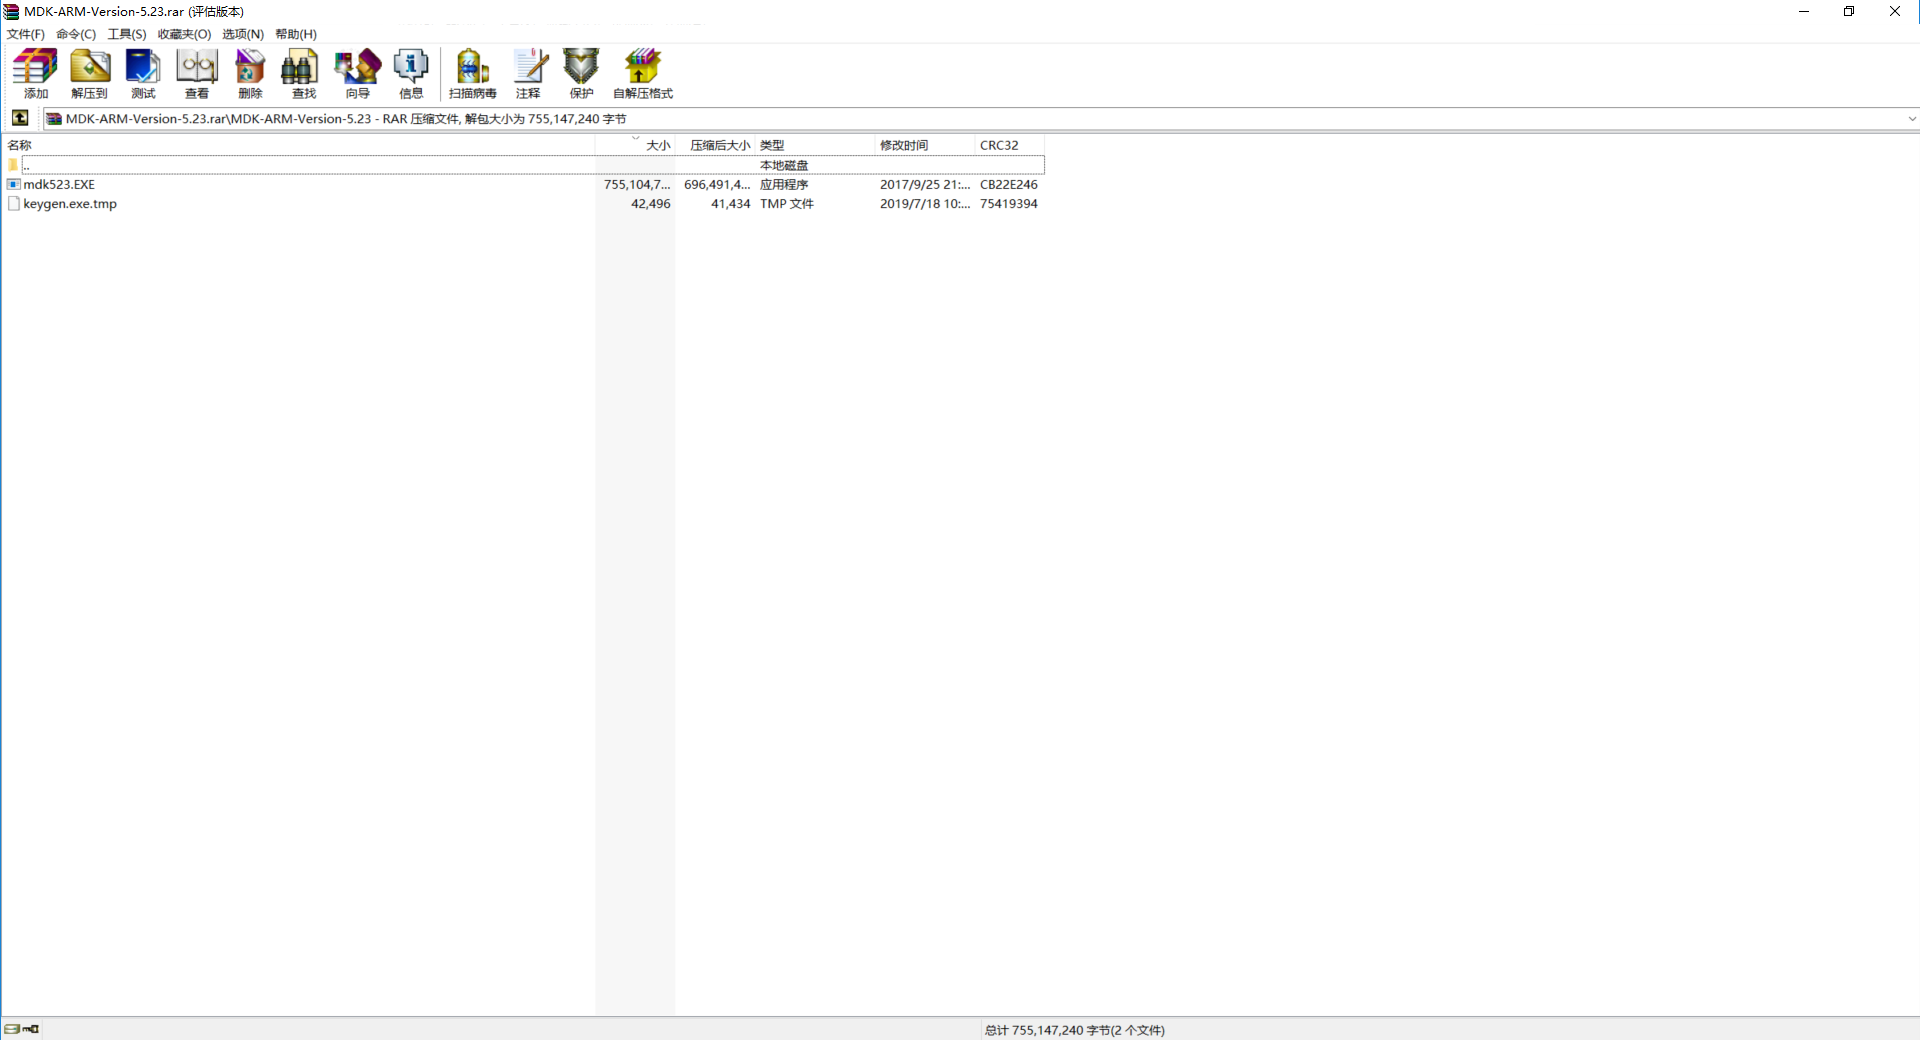
\includegraphics[width=1.0\textwidth]{ARMKeilMDKInstaller.png}
  \caption{ARM Keil MDK 安装包}
  \label{fig:ARMKeilMDKInstaller}
\end{figure}

按照正常流程安装 IDE 本体,安装完本体之后需要耐心等待一段时间更新下载相关的依赖,由于网络相关限制会出现更新下载超时的情况,需要手动点击继续保持持续更新。更新完之后可以看到 Nordic Semiconductor 公司的系列芯片设备及其对应的开发包。
\begin{figure}[htbp]
\centering
  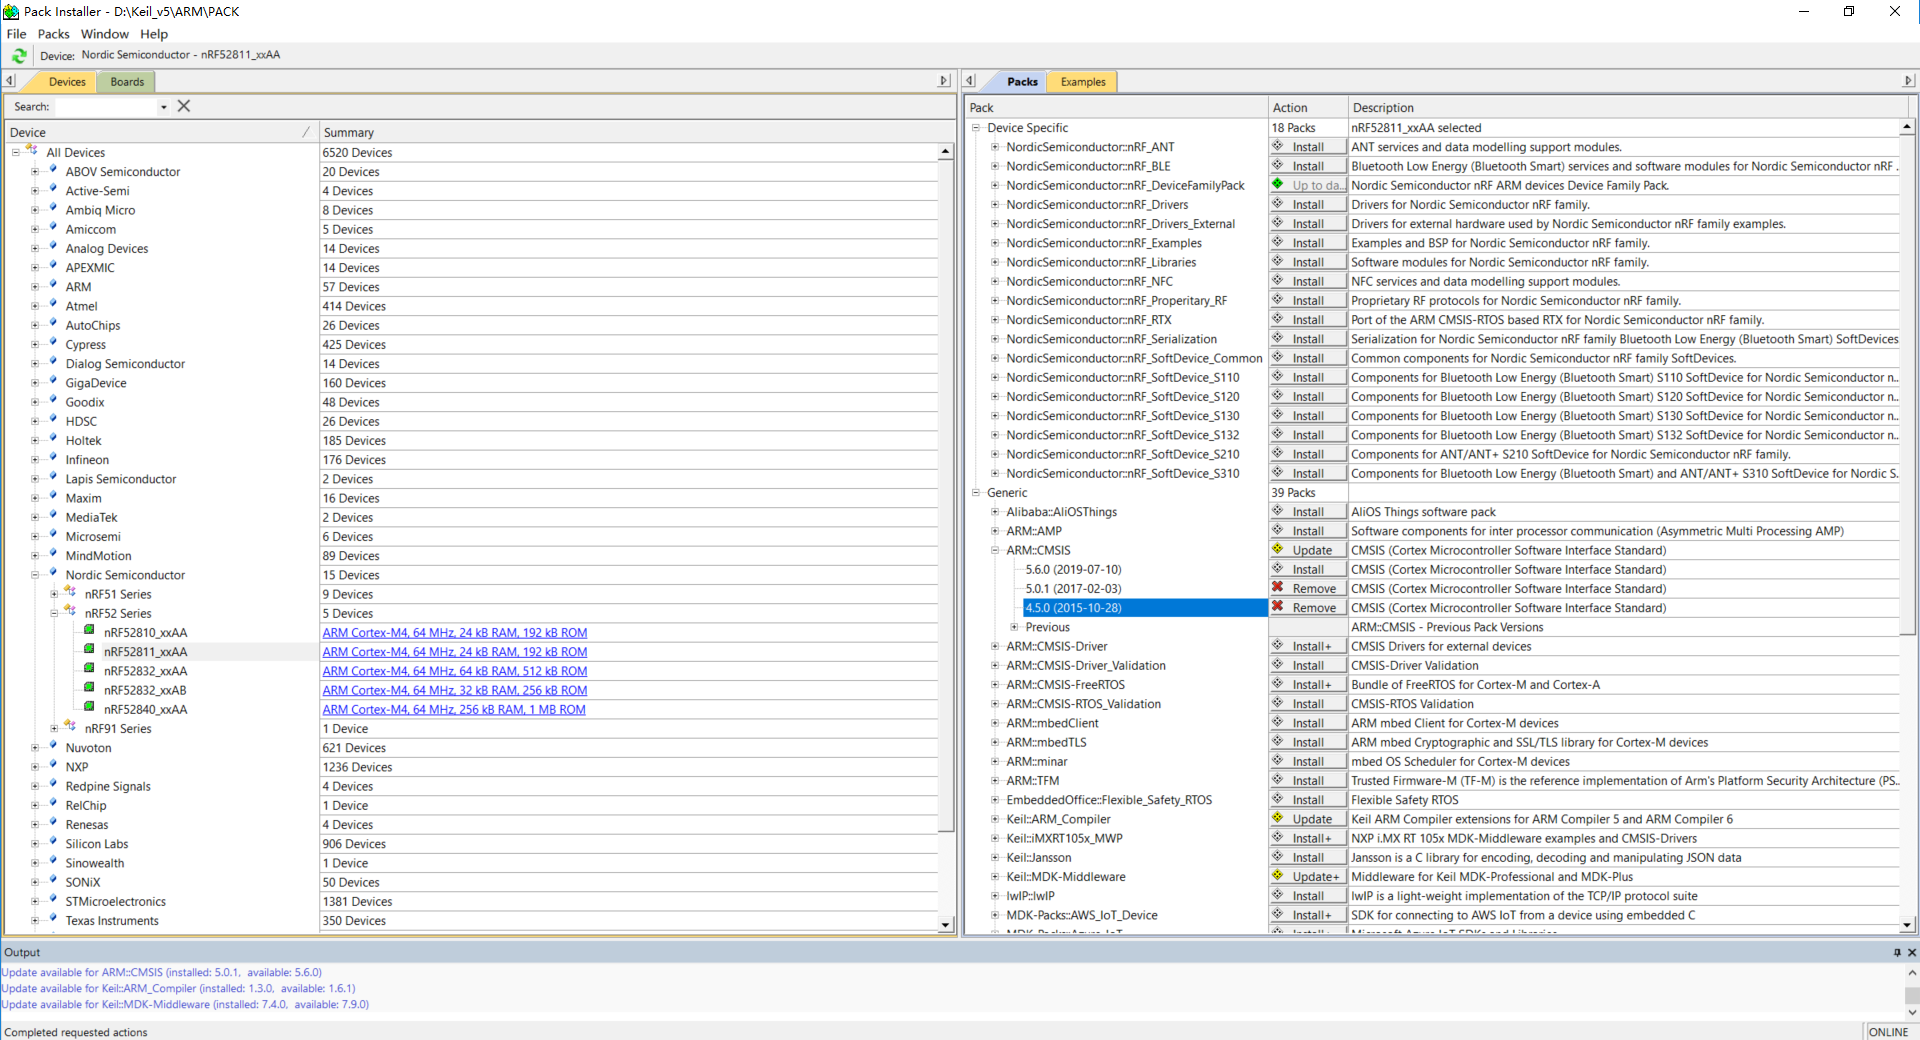
\includegraphics[width=1.0\textwidth]{ARMKeilPackInstaller.png}
  \caption{ARM Keil Software Packs 依赖包管理}
  \label{fig:ARMKeilPackInstaller}
\end{figure}

更新完相关依赖后使用注册机破解软件。首先 \textbf{以管理员身份运行} Keil uVision5,在文件菜单栏里打开许可证管理对话框;打开注册机;将 Computer ID 复制到 Keil Generic Keygen 对应的编辑栏中,Target 选择 ARM, 许可证选择 MDK Professional, 点击 Generate 按钮,生成 License ID Code(LIC); 将生成的许可证编号添加到许可证管理中,显示 Expires: Dec 2020,完成软件破解。
\begin{figure}[htbp]
\centering
  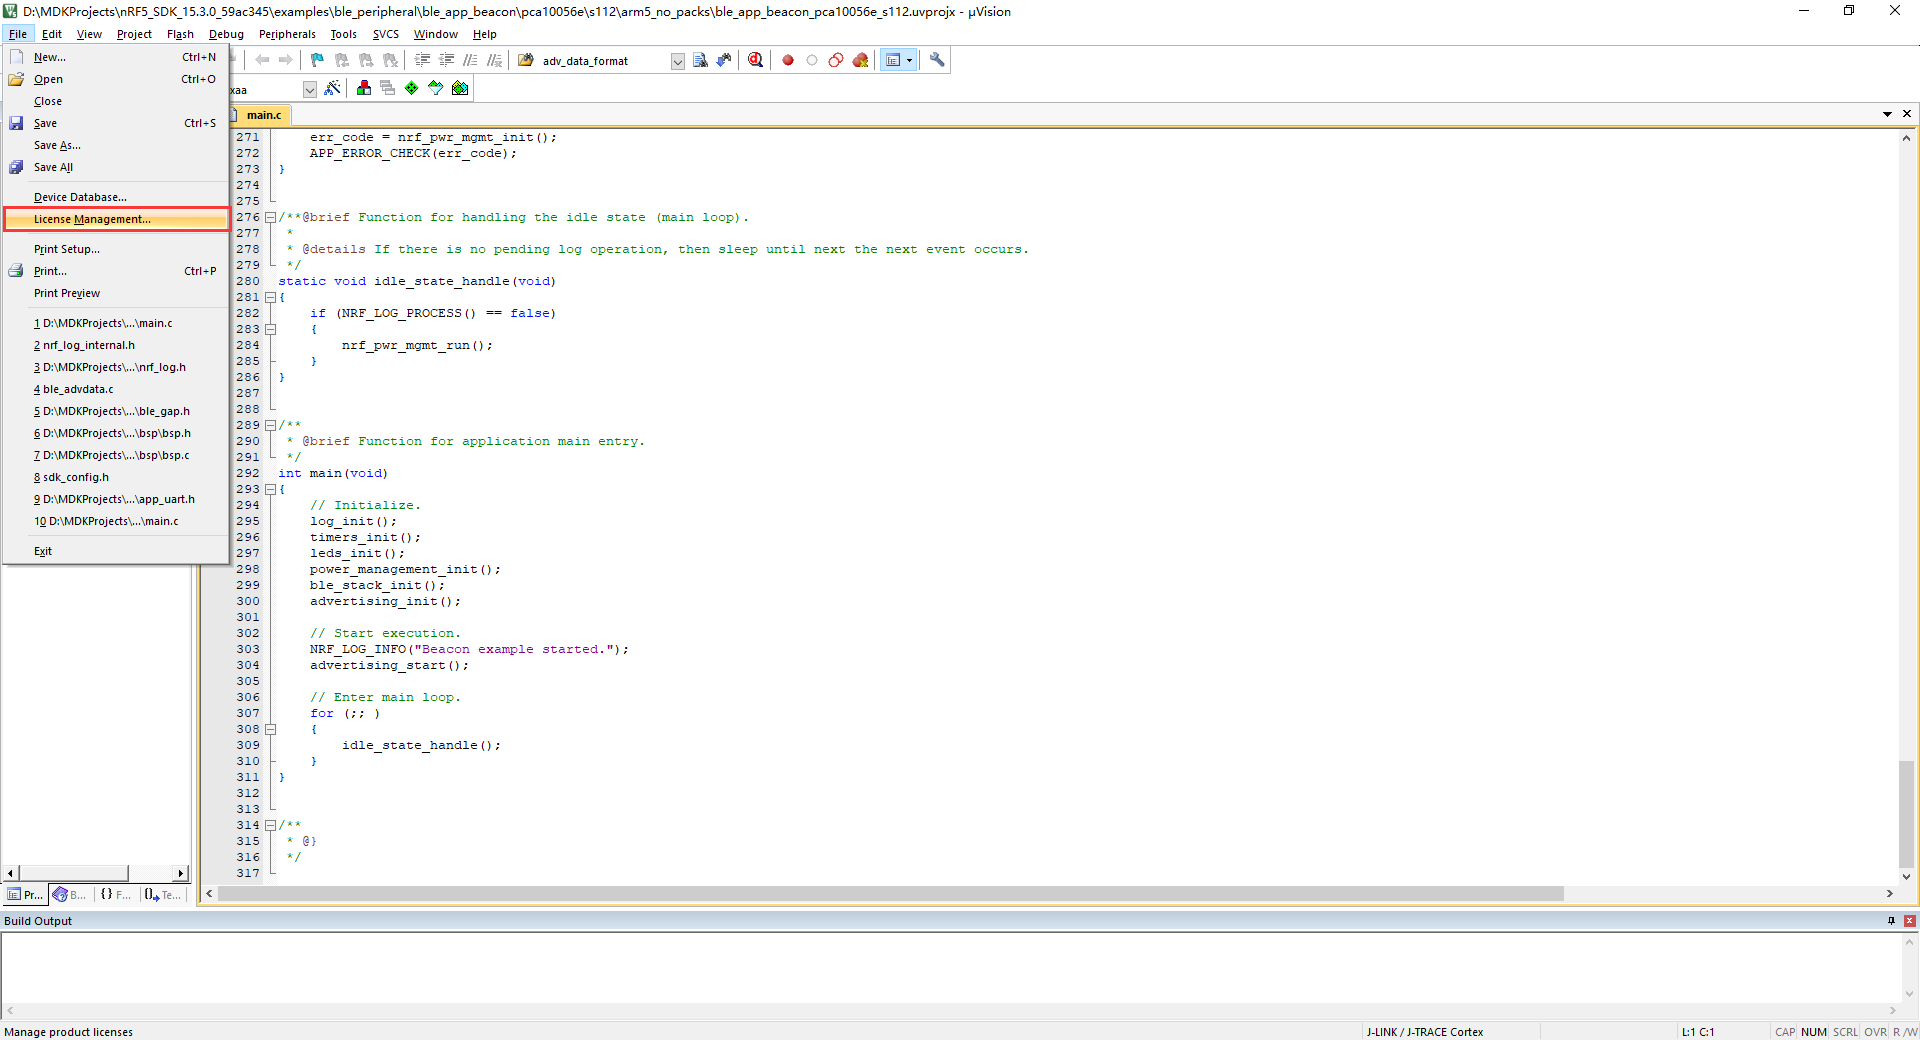
\includegraphics[width=1.0\textwidth]{ARMKeilMDKCracker1.png}
  \caption{ARM Keil 软件破解流程之打开License Management}
  \label{fig:ARMKeilMDKCracker1}
\end{figure}
\begin{figure}[htbp]
\centering
  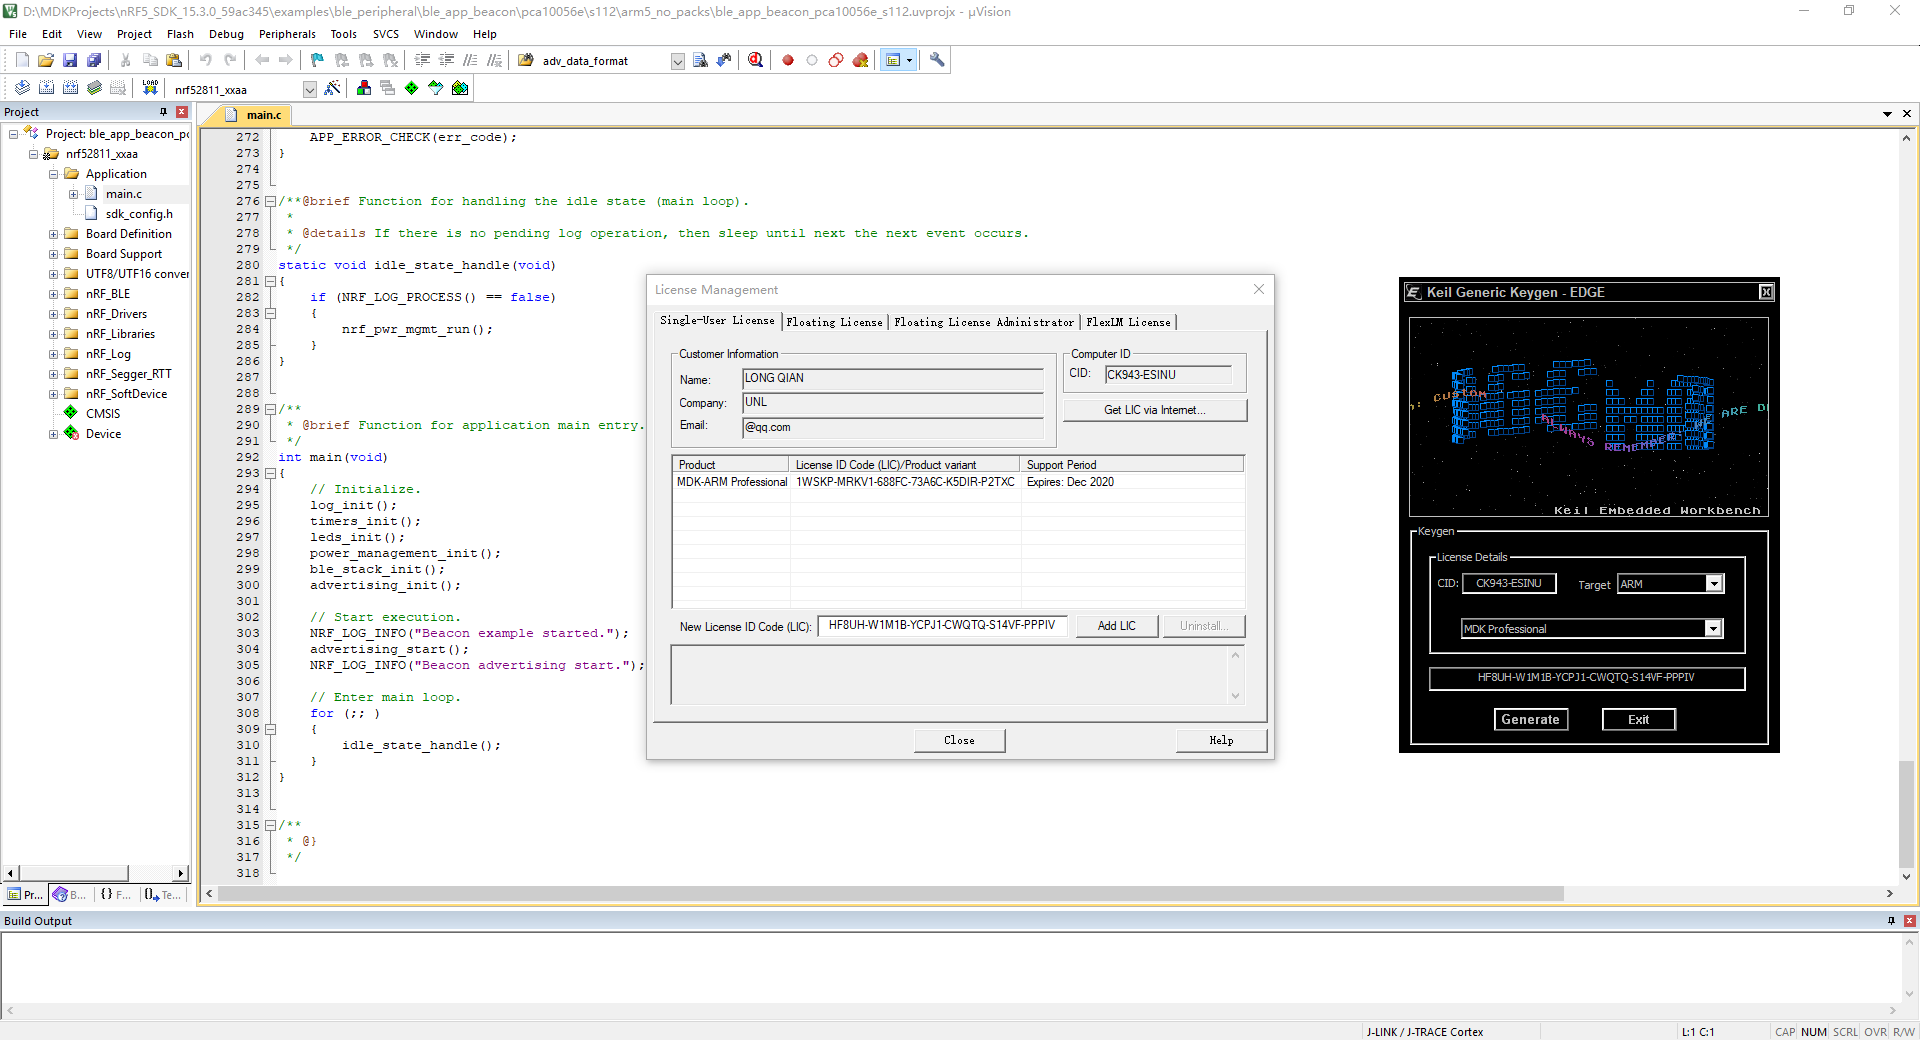
\includegraphics[width=1.0\textwidth]{ARMKeilMDKCracker2.png}
  \caption{软件破解流程之注册机生成LIC}
  \label{fig:ARMKeilMDKCracker2}
\end{figure}

$\star$ \href{https://developer.nordicsemi.com/}{nRF5 SDK}

nRF5 SDK 不需要安装,只需要在\href{https://www.nordicsemi.com/Software-and-Tools/Software/nRF5-SDK}{官方下载页面}下载最新的 SDK 即可,下载完毕之后解压出来即可使用。注意事项:nRF5 SDK 可能需要代理并且在网络状况较好的情况下才能完整下载下来;注意 SDK 解压出的文件夹的位置,因为 nRF5 SDK 中本身示例程序的文件路径较长,可能会导致编译器出现错误,所以尽量将 SDK 放置在靠近根目录的位置,避免路径中出现空格和中文字符。
\begin{figure}[htbp]
\centering
  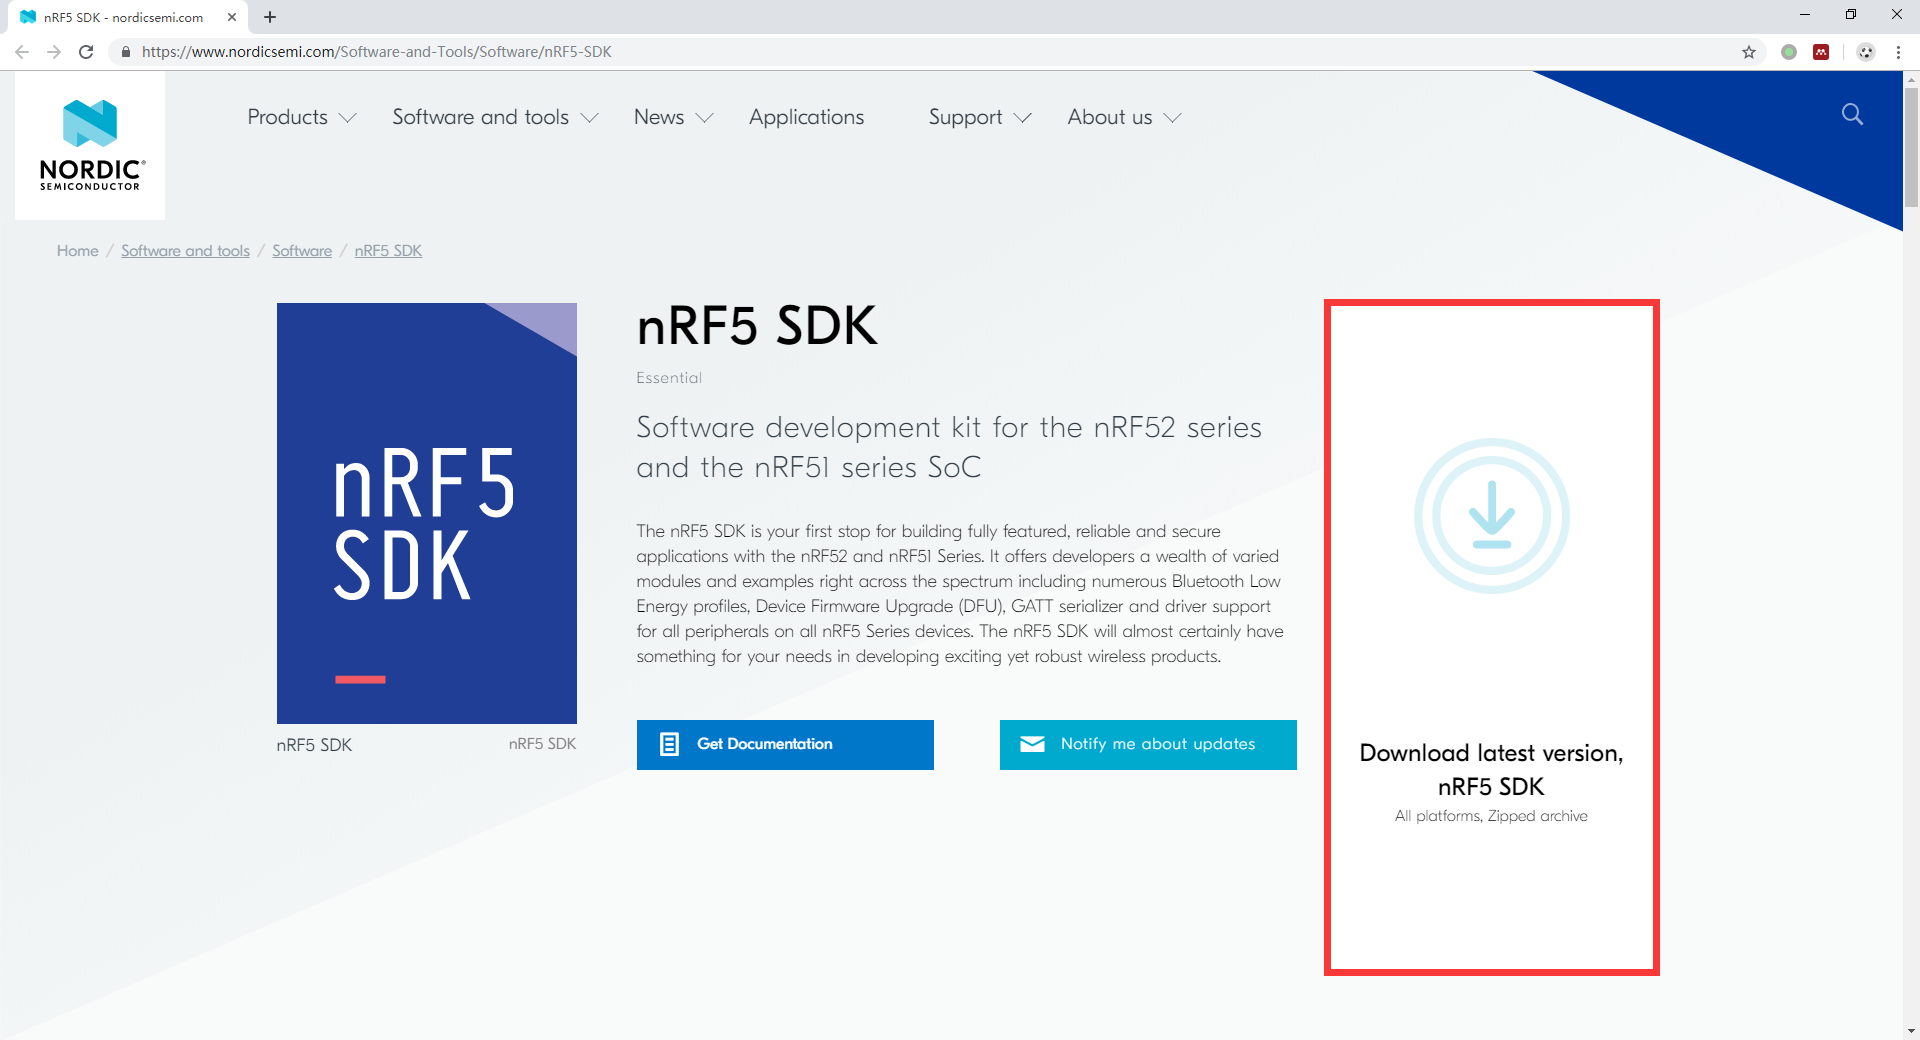
\includegraphics[width=1.0\textwidth]{nRF5SDKDownload.png}
  \caption{nRF5 SDK 下载}
  \label{fig:nRF5SDKDownload}
\end{figure}

$\star$ \href{https://www.nordicsemi.com/Software-and-Tools/Development-Tools/nRF5-Command-Line-Tools/Download#infotabs}{nRF5x Command Line Tools (including nrfjprog)}

nRF5x Command Line Tools 用于开发、编程和调试 Nordic Semiconductor 公司的 nRF5x 系列 SoCs。同样在\href{https://www.nordicsemi.com/Software-and-Tools/Development-Tools/nRF-Command-Line-Tools/Download}{官方下载页面}下载对应操作系统的安装包,按照安装指引完成 nRF 命令行工具的安装。在 Powershell 中输入命令 \textit{nrfjprog --version},验证 nrfjprog 安装正确。
\begin{figure}[htbp]
\centering
  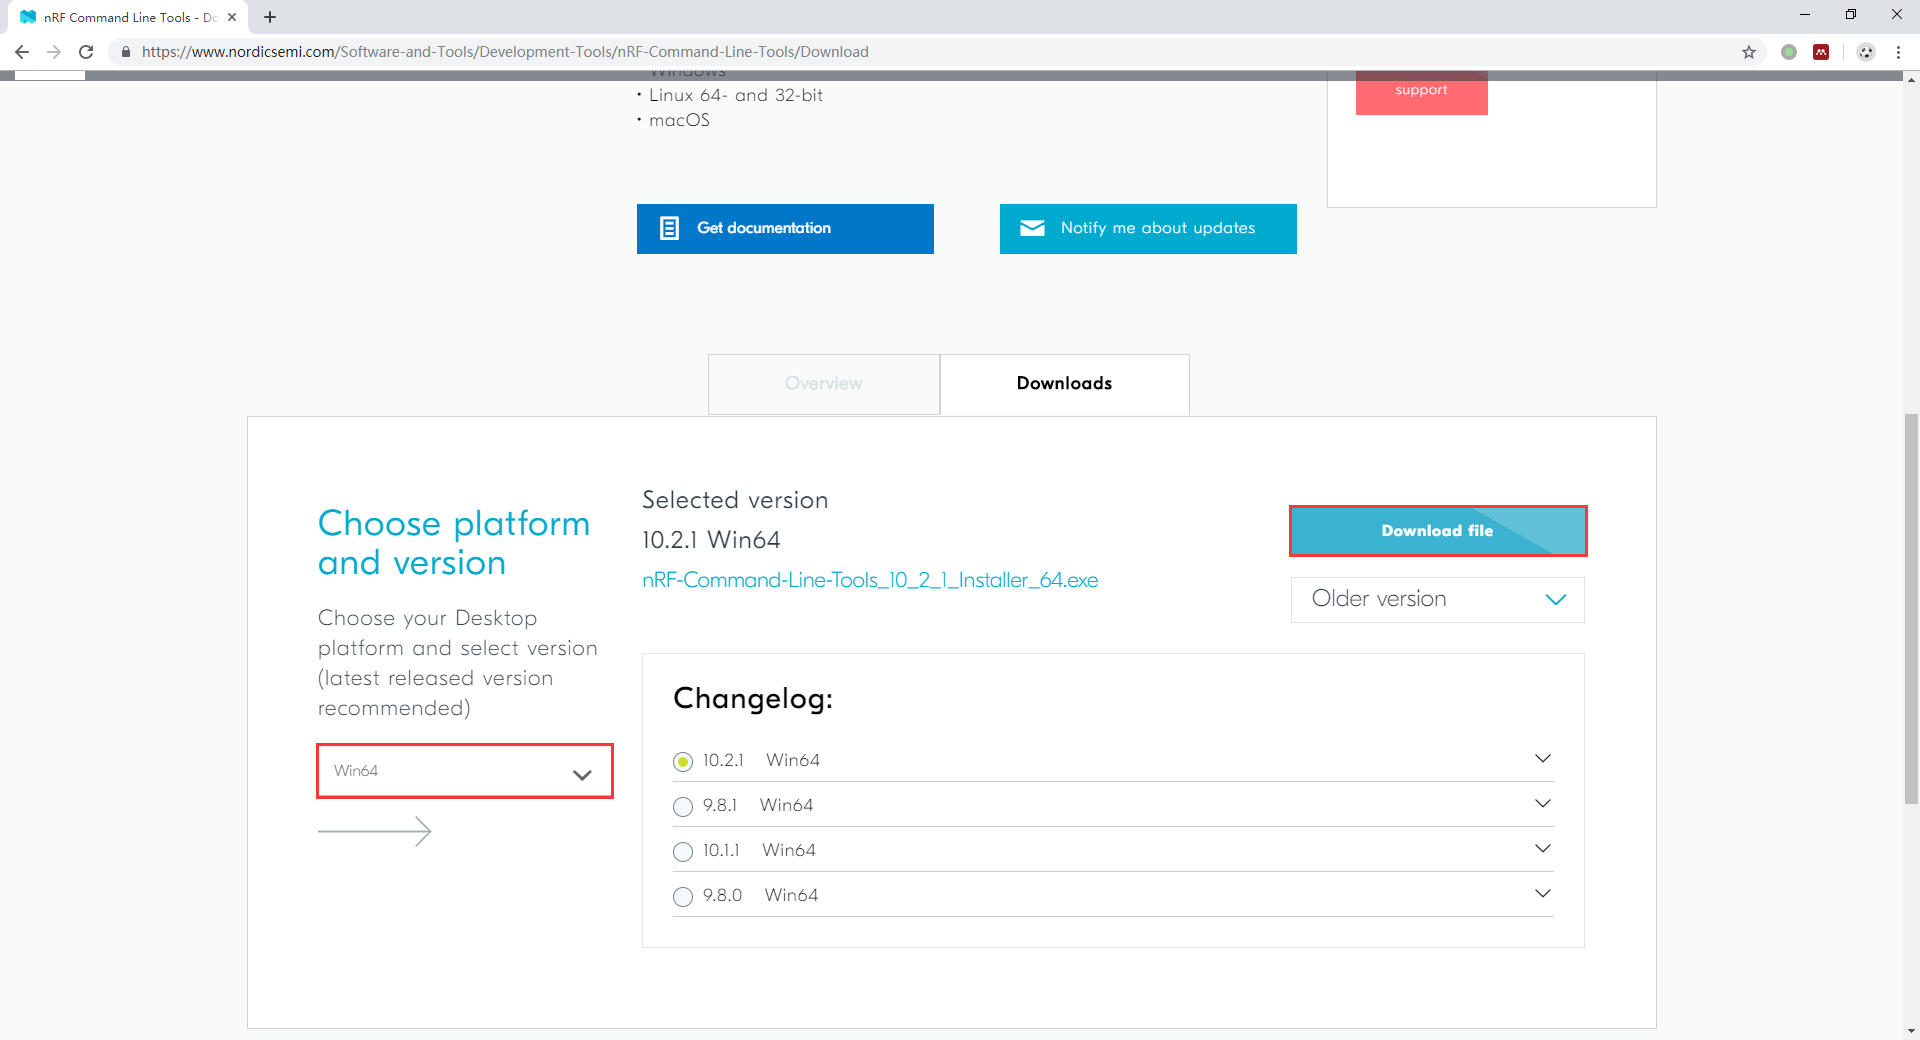
\includegraphics[width=1.0\textwidth]{nRFCLTDownload.png}
  \caption{nRF Command Line Tools 下载}
  \label{fig:nRFCLTDownload}
\end{figure}

\begin{figure}[htbp]
\centering
  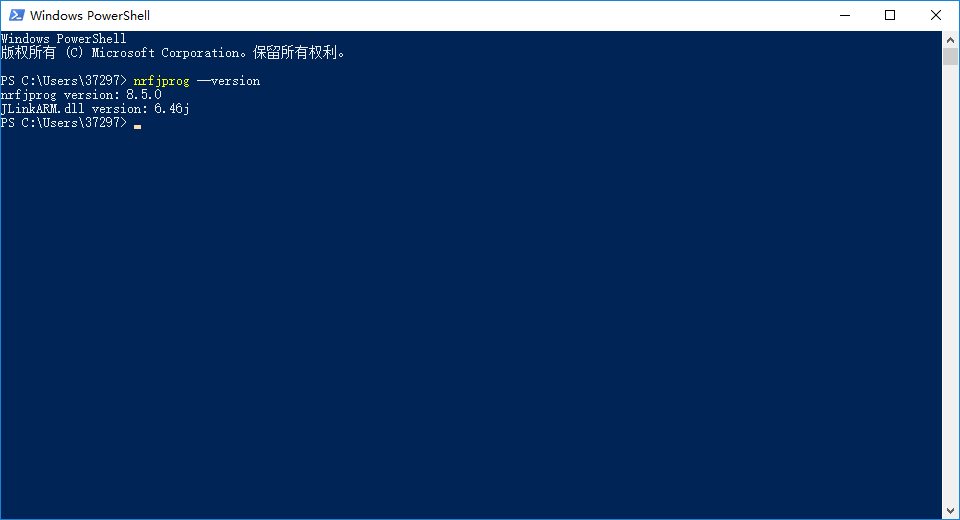
\includegraphics[width=1.0\textwidth]{nRFCLTValidation.png}
  \caption{nRF Command Line Tools 验证安装}
  \label{fig:nRFCLTValidation}
\end{figure}

$\bigstar$ 可选安装项

\subsection{\href{https://infocenter.nordicsemi.com/index.jsp?topic=\%2Fug_gsg_keil\%2FUG\%2Fgsg\%2Finstall_nrf5_sdk.html}{编写嵌入式程序(Programming an application)}}

完成上节工具链配置后就可以开始嵌入式程序的编写,在 Windows 平台,本节采用图形界面烧制程序。嵌入式程序的烧制大致分为以下四个步骤。

$\bigstar$ \href{https://infocenter.nordicsemi.com/index.jsp?topic=\%2Fug_gsg_keil\%2FUG\%2Fgsg\%2Ferase_board.html}{擦除开发板(Erasing the board)}

官方教程给出可以通过命令行或者 nRFgo Studio 擦除闪存,但是打开 nRFgo Studio 并没有在Device Manager里找到自定义开发版的信息,所以暂时没有办法采用该方式擦除闪存。在叶博的指导下,通过 J-Link 软件包中的 J-Flash Lite 软件可以确实擦除闪存。
\begin{figure}[htbp]
\centering
  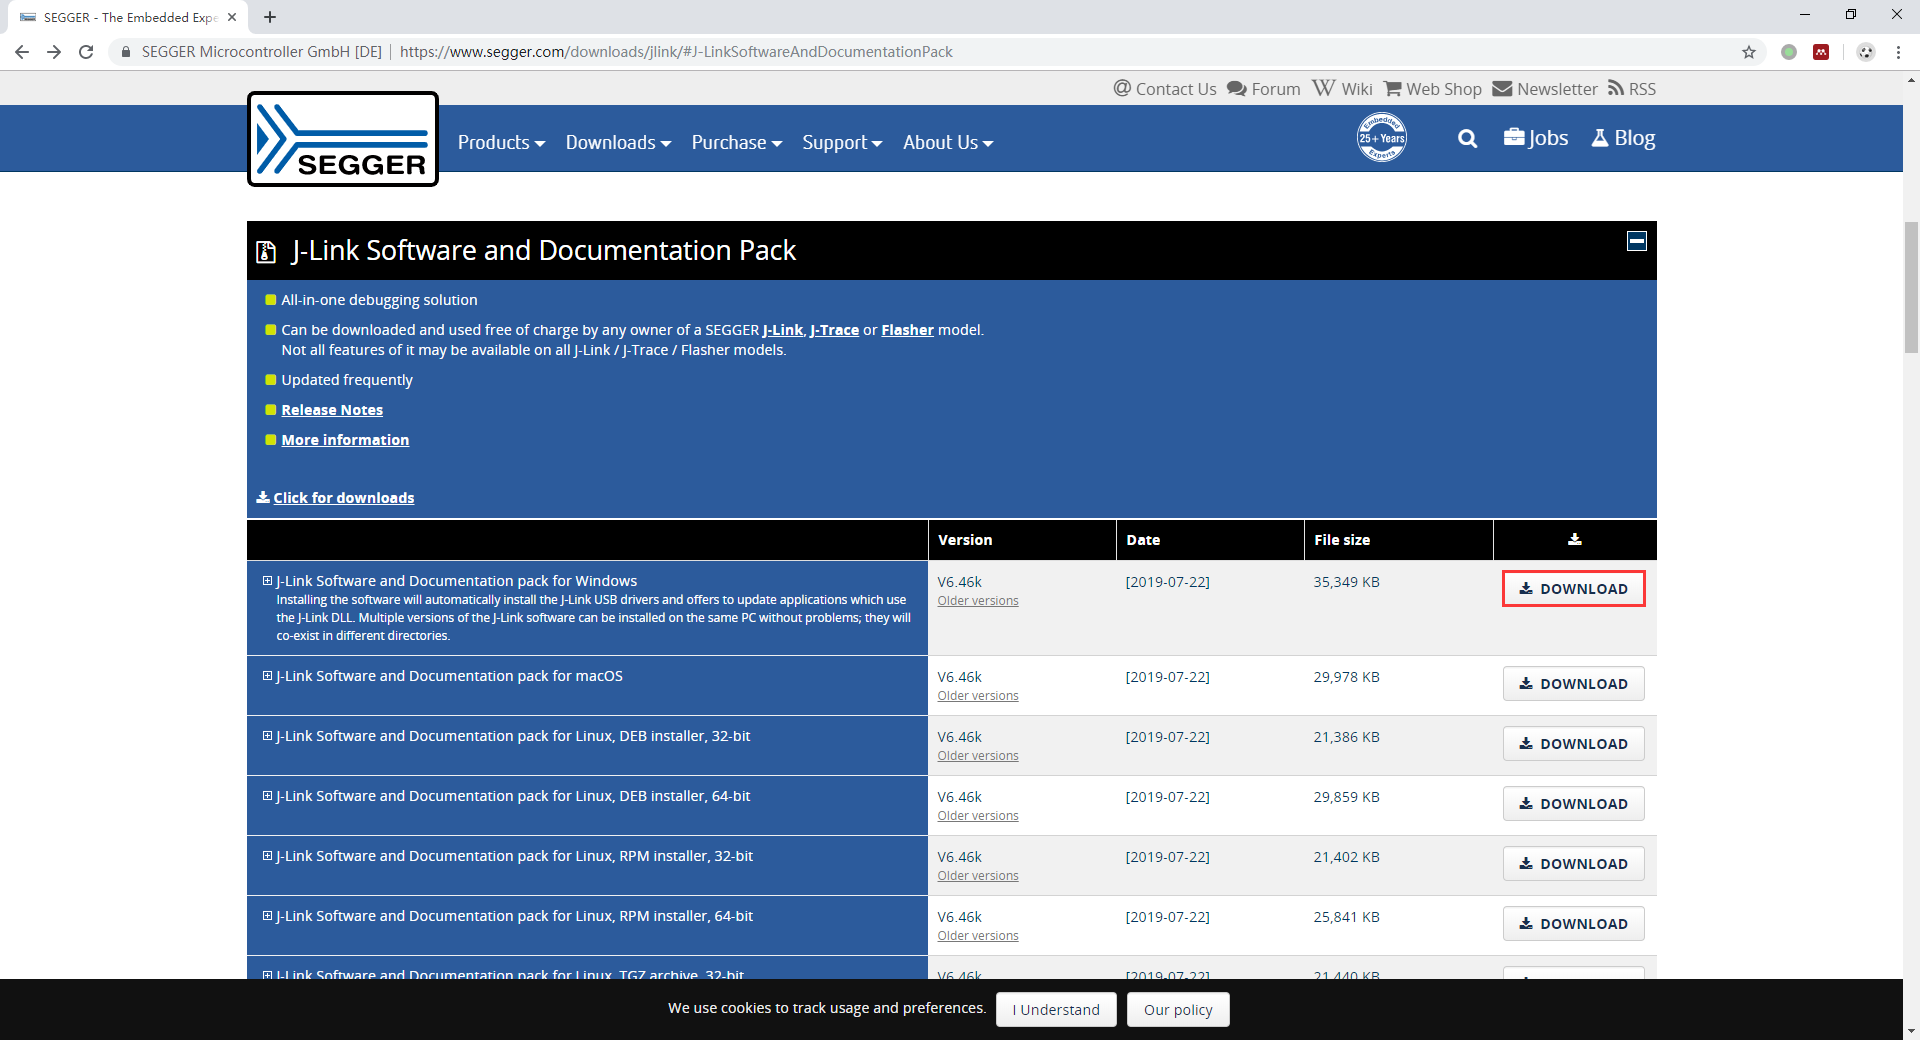
\includegraphics[width=1.0\textwidth]{J-LinkSoftwareDownload.png}
  \caption{J-Link 软件包下载}
  \label{fig:J-LinkSoftwareDownload}
\end{figure}

\begin{figure}[htbp]
	\centering
	\begin{subfigure}[htbp]{1.0\textwidth}
	\centering
		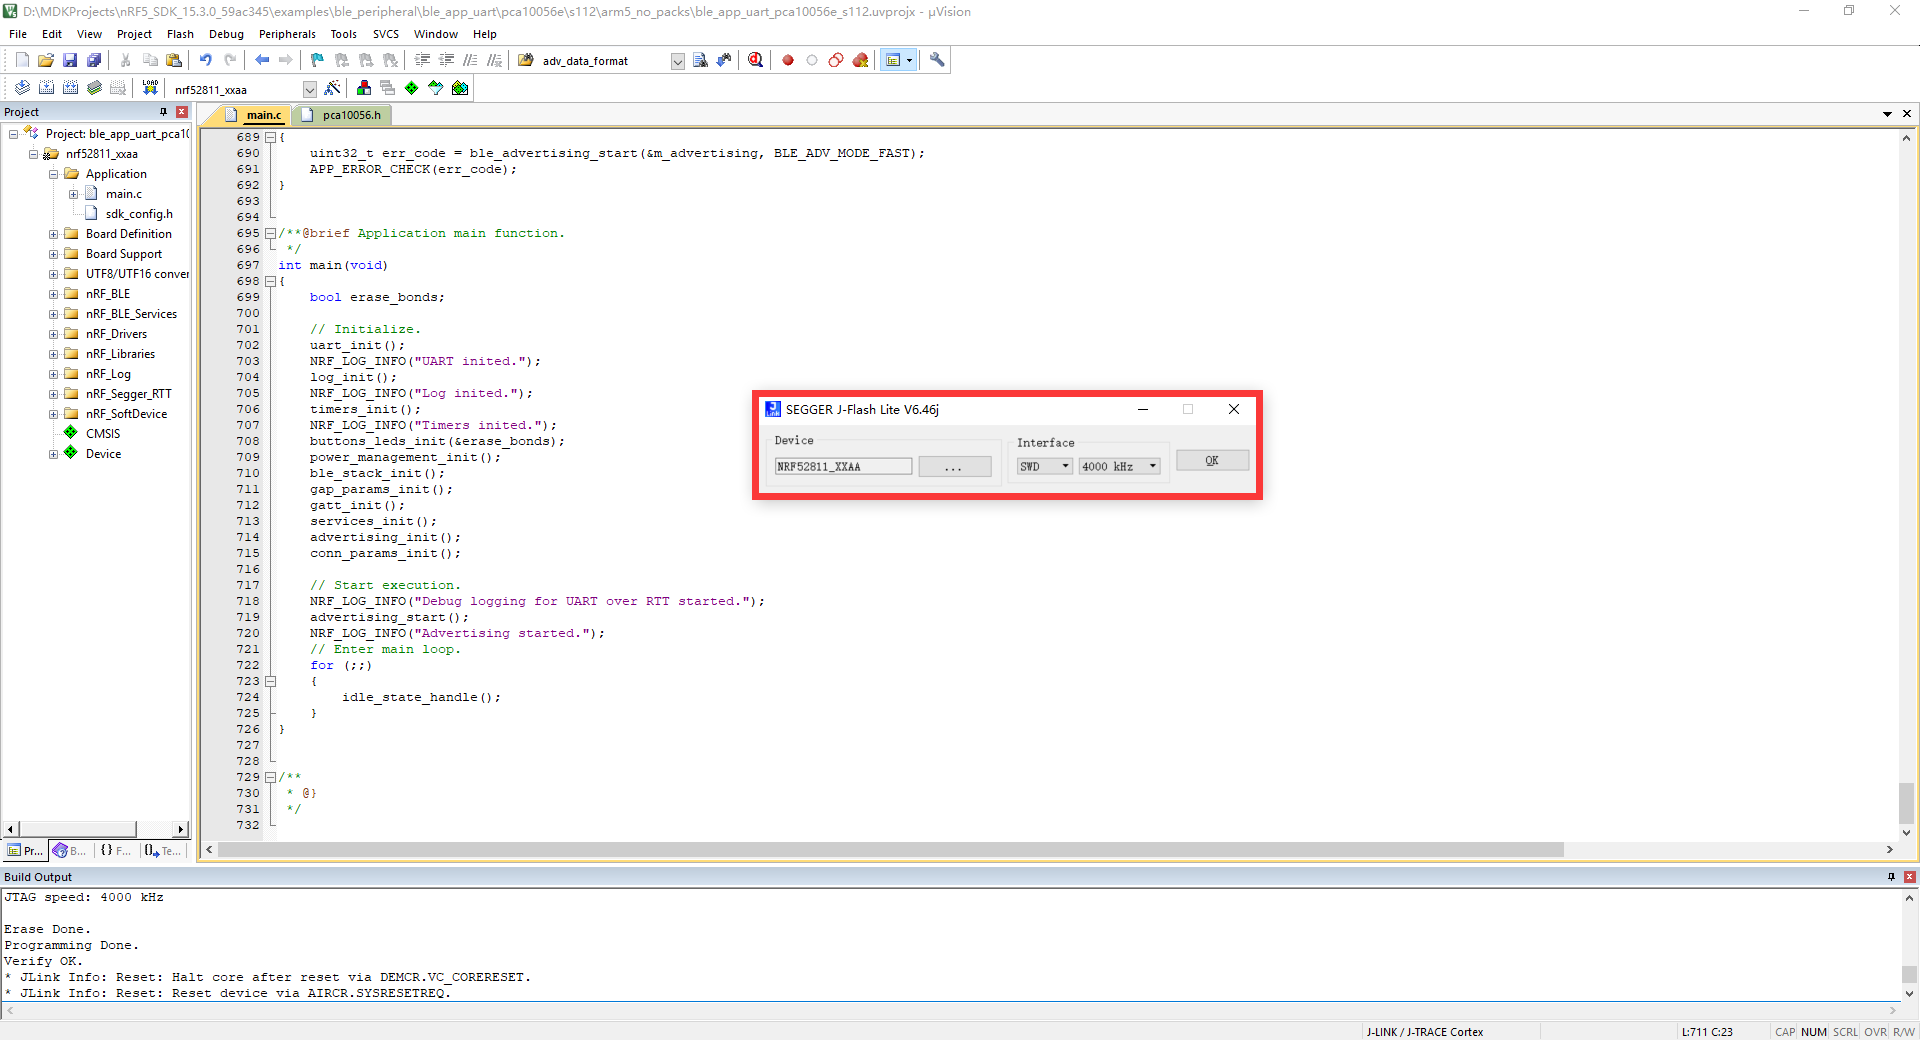
\includegraphics[width=.9\textwidth]{SEGGERJ-FlashLiteV6-46j.png}
		\label{fig:SEGGERJ-FlashLiteV6.46j}
		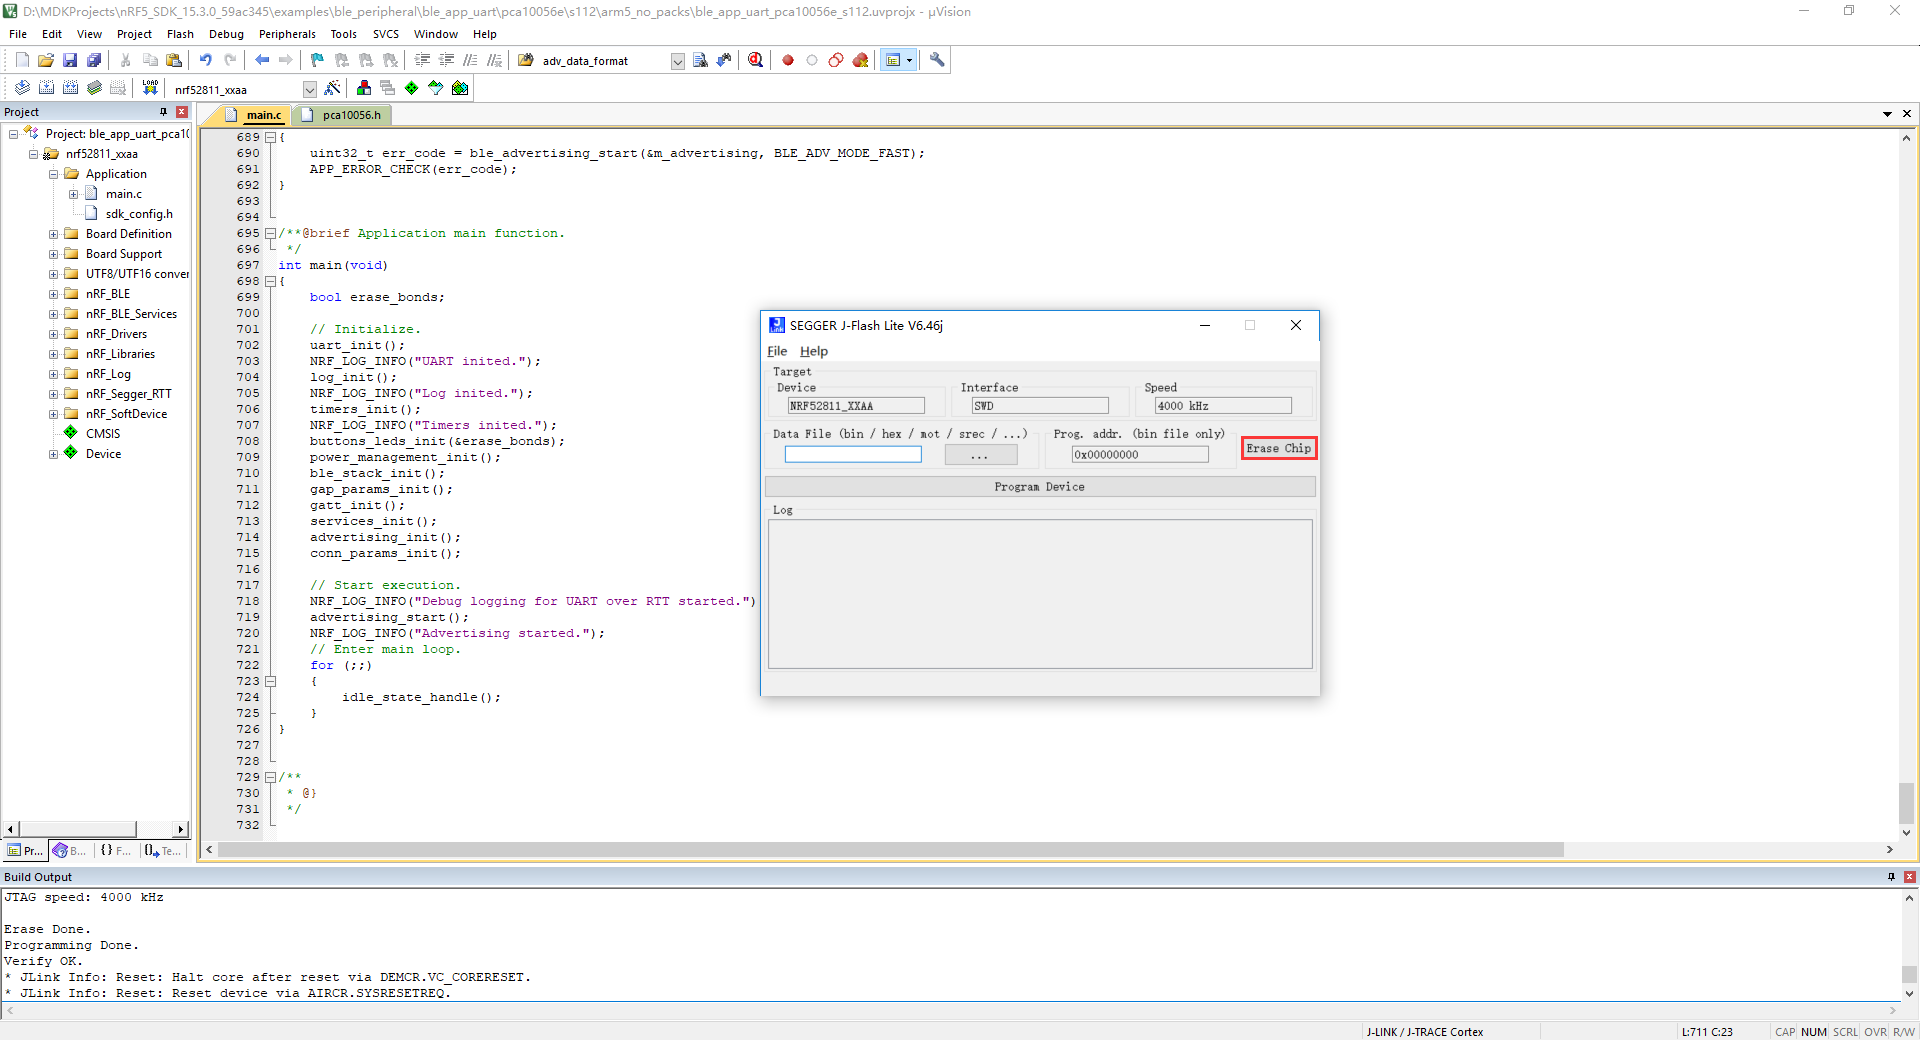
\includegraphics[width=.9\textwidth]{SEGGERJ-FlashLiteV6-46j-EraseChip.png}
		\label{fig:SEGGERJ-FlashLiteV6.46j-EraseChip}
	\end{subfigure}
	\caption{SEGGER J-Flash Lite V6.46j 擦除闪存}
	\label{fig:SEGGERJ-FlashLite}
\end{figure}

$\bigstar$ \href{https://infocenter.nordicsemi.com/index.jsp?topic=\%2Fug_gsg_keil\%2FUG\%2Fgsg\%2Fcompile_keil.html}{编译应用程序(Compiling the application)}

在 nRF5 SDK 中提供了 Keil µVision 示例程序,根据自定义板卡的基础配置,进行简单的配置修改即可完成嵌入式程序的编译。对于基于 nRF52811 芯片的开发,还需要参考对应这款芯片的 \href{https://infocenter.nordicsemi.com/index.jsp?topic=\%2Fstruct_nrf52\%2Fstruct\%2Fnrf52811.html&cp=3_2}{开发文档 Developing for nRF52811}。在 SDK 中包含官方提供的针对不同板卡和蓝牙协议栈的示例工程代码,存放在以下路径。

{\setmainfont{Courier New Italic}                          % 设置代码字体                   
\begin{lstlisting}
SDK_dir\examples\ble_peripheral\ble_app_uart\board\SoftDevice
\arm5_no_packs
\end{lstlisting}}

官方教程选用了 \textit{ble\textunderscore app\textunderscore uart} 作为示例,对于 nRF52811 开发板,打开下面路径下的工程文件 \textit{ble\textunderscore app\textunderscore uart\textunderscore pca10056e\textunderscore s112.uvprojx},如果 IDE 提示安装 \textit{nRF\textunderscore DeviceFamilyPack} 的相关依赖,选择接收并安装 \textit{Device Family Pack}。

{\setmainfont{Courier New Italic}                          % 设置代码字体                   
\begin{lstlisting}
SDK_dir\examples\ble_peripheral\ble_app_uart\pca10056e\s112
\arm5_no_packs
\end{lstlisting}}

在 nRF52811 的开发文档中提到, nRF SDK中,目前并没有为 nRF52811 提供专门的开发包,需要用 nRF52840 的开发包模拟 nRF52811 上的相关功能,进而完成 nRF52811 的开发。从 nRF SDK V15.3.0 开始,支持 nRF52811 SoC 在 PCA10056 开发板上进行开发(原本是 nRF52840 对应的开发板),即可以将 nRF52811 视为 nRF52840 的子集,相比 nRF52840,nRF52811 开发板上的资源相对受限,内存、闪存和外围设备资源更少,所以在进行开发时需要对预设的开发板配置进行修改,从而使得程序能够原生的运行在 nRF52811 开发板上。这里要特别注意的是示例程序是以 pca10056 开发板作为配置电路板,需要根据自己构建的板卡重新定义相关引脚,从而使得 UART 串口能正常通信。
\begin{figure}[htbp]
\centering
  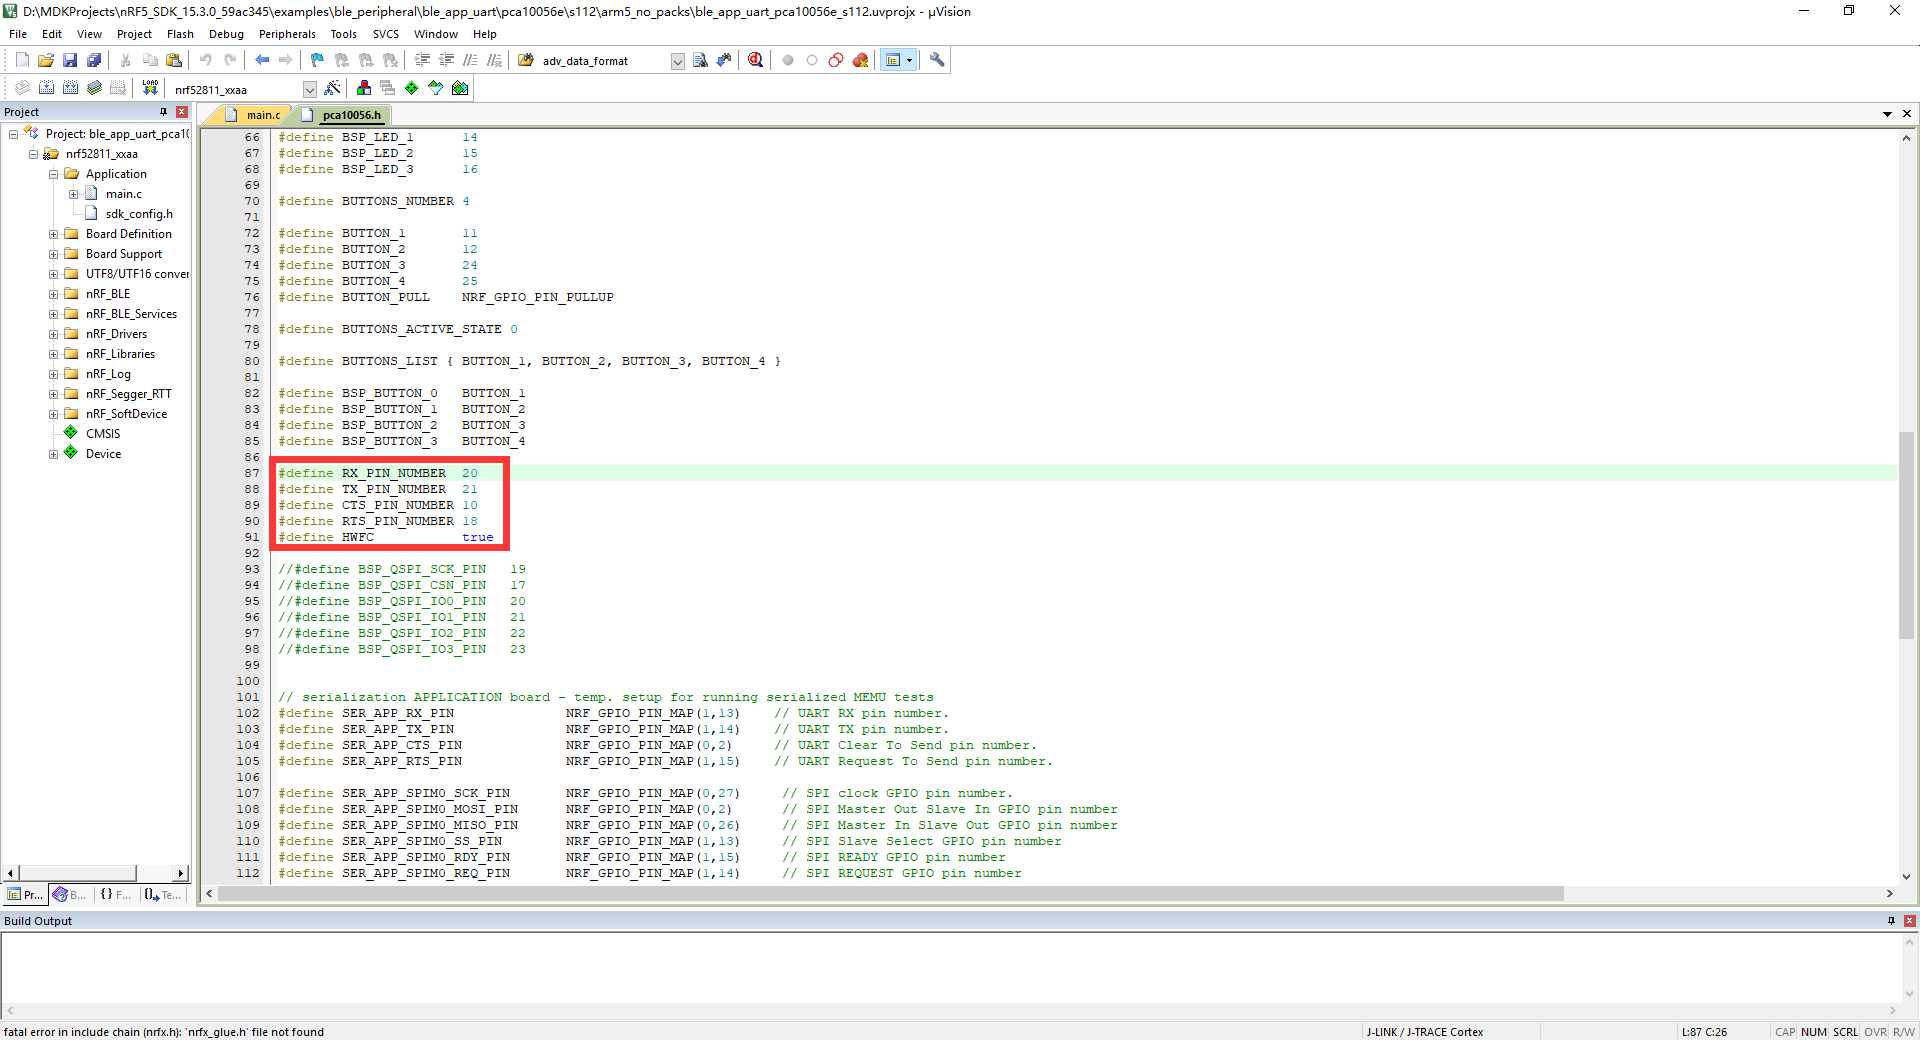
\includegraphics[width=1.0\textwidth]{PCA10056PIN.png}
  \caption{PCA10056 适配自定义引脚}
  \label{fig:PCA10056PIN}
\end{figure}

$\bigstar$ \href{https://infocenter.nordicsemi.com/index.jsp?topic=\%2Fug_gsg_keil\%2FUG\%2Fgsg\%2Fprogram_sd.html}{烧制蓝牙协议栈(Programming the SoftDevice)}

如果编写的嵌入式程序中使用了 Bluetooth\textsuperscript{\textregistered} 或者 ANT\textsuperscript{\texttrademark},这里需要重点强调,在烧制嵌入式程序之前,需要首先将蓝牙协议栈烧制进板卡中,在 Keil 中切换烧制对象,点击下载(LOAD)按钮,即可完成蓝牙协议栈的烧制。
\begin{figure}[htbp]
\centering
  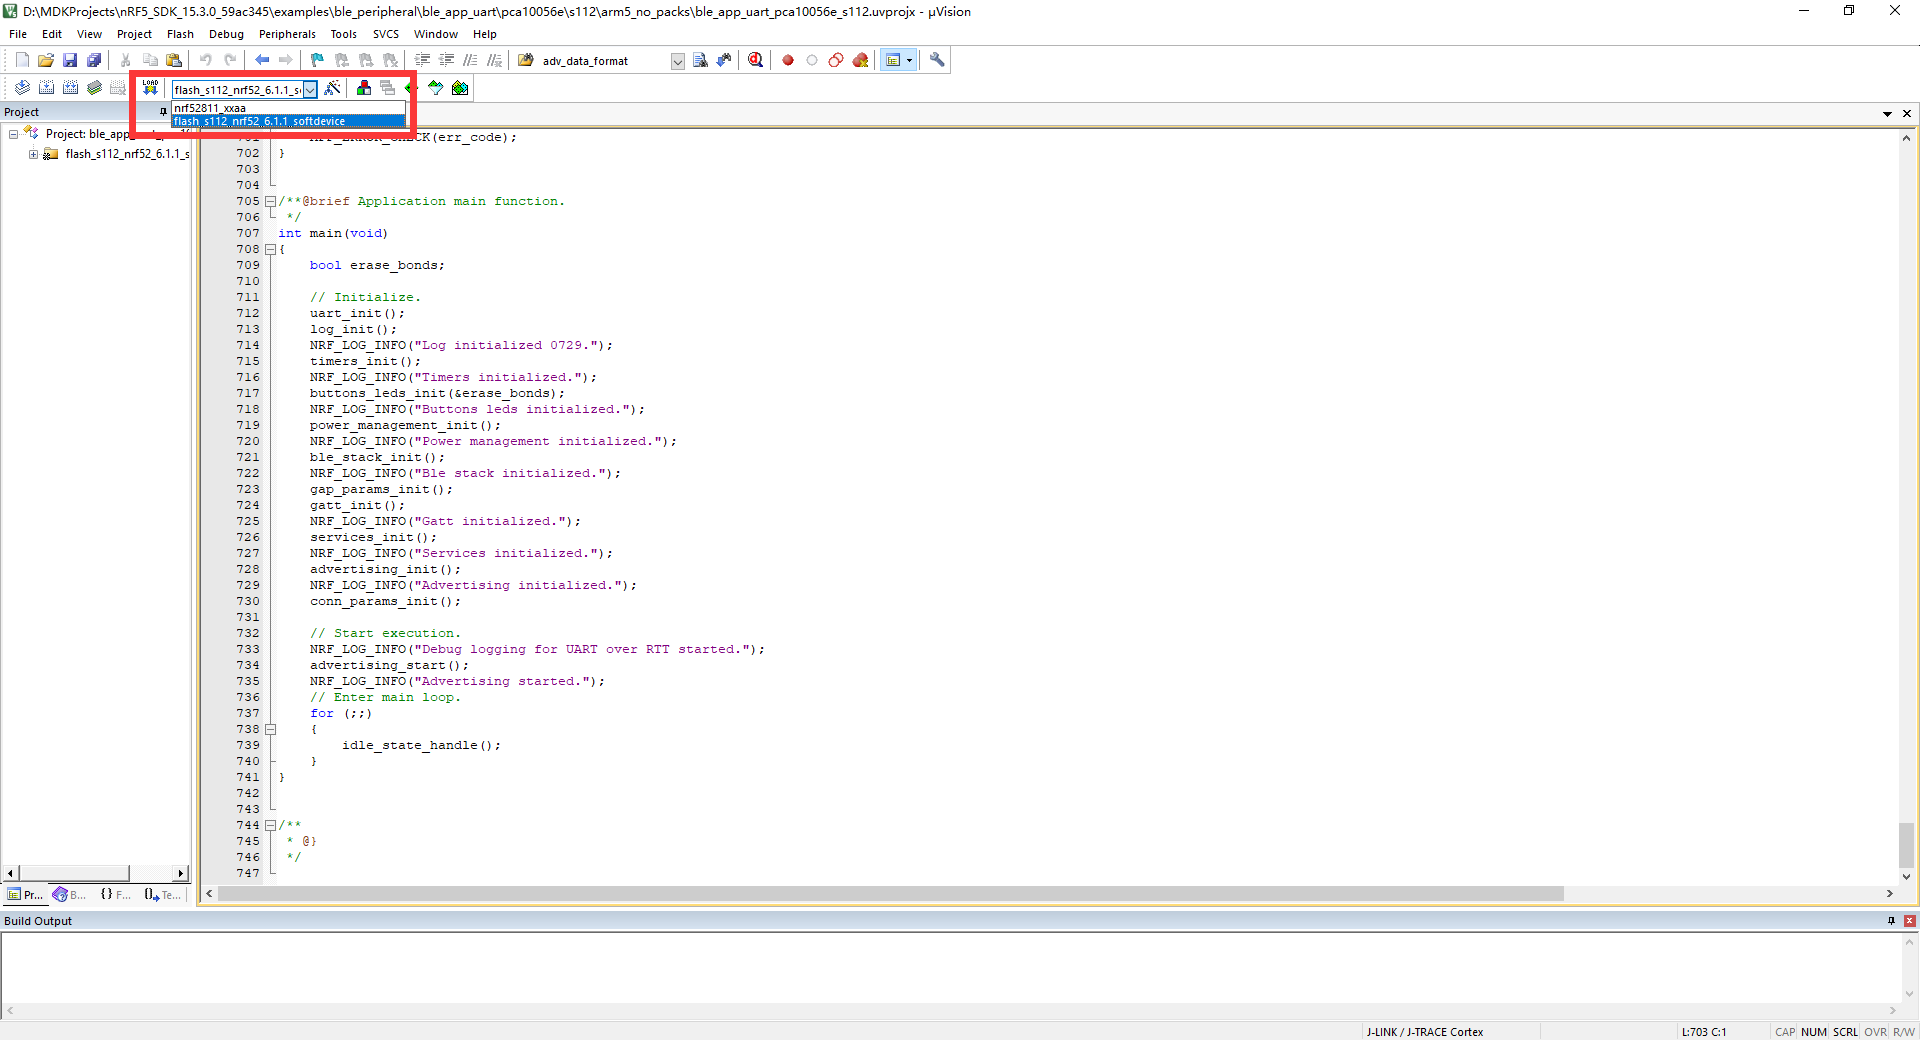
\includegraphics[width=1.0\textwidth]{FlashSoftDevice.png}
  \caption{烧制蓝牙协议栈}
  \label{fig:FlashSoftDevice}
\end{figure}

$\bigstar$ \href{https://infocenter.nordicsemi.com/index.jsp?topic=\%2Fug_gsg_keil\%2FUG\%2Fgsg\%2Fprogram_app_keil.html}{烧制应用程序(Programming the application)}

同烧制蓝牙协议栈类似,在完成嵌入式程序编译后,将烧制目标切换为对应芯片,点击下载(LOAD)按钮,即可完成应用程序的烧制。

\subsection{\href{https://infocenter.nordicsemi.com/index.jsp?topic=\%2Fug_gsg_keil\%2FUG\%2Fgsg\%2Fcommunicate.html&cp=1_1_1_8}{建立开发板通讯(Communicating with the board)}}

为了在电脑上显示应用程序开发中的打印信息或者向应用程序发送指令,需要与开发板进行通讯。官方建议采用 SEGGER Real Time Transfer (RTT) 技术,相比于 Universal Asynchronous Receiver/Transmitter (UART) 通讯, RTT 不需要占用额外的针脚,通过 J-Link 调试接口,即可实现 PC 和开发板的双向通信。

\subsection{\href{https://infocenter.nordicsemi.com/index.jsp?topic=\%2Fug_gsg_keil\%2FUG\%2Fgsg\%2Ftest.html&cp=1_1_1_9}{测试嵌入式程序(Testing the application)}}


%%%=== 参考文献 ========%%%
\cleardoublepage\phantomsection
\addcontentsline{toc}{chapter}{参考文献}
\begin{thebibliography}{000}\zihao{5}

  \bibitem{BKY_iini} 博客园.Nordic nRF51/nRF52开发环境搭建[Z].iini,2018.  
  
\end{thebibliography}

\cleardoublepage
\end{document}



